\documentclass[conference]{IEEEtran}

\ifCLASSINFOpdf
   \usepackage[pdftex]{graphicx}
  % declare the path(s) where your graphic files are
   \graphicspath{{../pdf/}{../jpeg/}}
  % and their extensions so you won't have to specify these with
  % every instance of \includegraphics
   \DeclareGraphicsExtensions{.pdf,.jpeg,.png}
\else
  % or other class option (dvipsone, dvipdf, if not using dvips). graphicx
  % will default to the driver specified in the system graphics.cfg if no
  % driver is specified.
  \usepackage[dvips]{graphicx}
  % declare the path(s) where your graphic files are
  \graphicspath{{../eps/}}
  % and their extensions so you won't have to specify these with
  % every instance of \includegraphics
  \DeclareGraphicsExtensions{.eps}
\fi


\usepackage[utf8x]{inputenc}
\usepackage[T1]{fontenc}
\usepackage{lmodern}
\usepackage{booktabs}
\usepackage{multirow}
\usepackage{algorithmic}
\usepackage[Algoritmo]{algorithm}
\usepackage[spanish,USenglish]{babel}
\usepackage[colorlinks=true,linkcolor=black,urlcolor=black,citecolor=black, urlcolor=black, filecolor=black bookmarks=false]{hyperref}
\usepackage{subfigure}


\addto\captionsspanish{
 \def\tablename{Tabla}}


\begin{document}

\pagestyle{empty}  

\selectlanguage{spanish}

\title{Biomass}

\author{\IEEEauthorblockN{GIEE}
\IEEEauthorblockA{Universidad de Nariño\\
San Juan de Pasto, Colombia\\
Email: }
\and
\IEEEauthorblockN{GIIWW}
\IEEEauthorblockA{Universidad de Nariño\\
San Juan de Pasto, Colombia\\
Email: }
}

\maketitle

\selectlanguage{USenglish}
\begin{abstract}

En este artículo se describen los componentes básicos que conforman
la investigación aplicada que tiene como objetivo la construcción de un
primer mapa del potencial de biomasa en el departamento de Nariño a
partir de imágenes satelitales Landsat de libre acceso. En el cual se 
analizan las diferentes bandas de las imágenes satelitales disponibles y
su relación con la biomasa aplicando técnicas de regresión y obteniendo un modelo
para la generación de mapas en el departamento de Nariño.

\end{abstract}
 
\selectlanguage{spanish}


\begin{IEEEkeywords}
biomass, regression models 
\end{IEEEkeywords}

\thispagestyle{empty} 

\IEEEpeerreviewmaketitle


\section{Introducción}

\IEEEPARstart Según estudios del Ministerio de Minas y Energía de Colombia, en el departamento de Nariño hay 15 municipios con cobertura eléctrica inferior al 80\% \cite{ministerio_de_minas_y_energia_plan_2008}. Como nueva estratégia para enfrentar esta problemática se ha planteado la medición y estimación de potenciales energéticos en las zonas más viables de la región. Uno de los componentes a analizar es el potencial de biomasa para la generación eléctrica. Sin embargo, uno de los problemas que se plantea para la ubicación de lugares propicios es la ausencia de bases de datos actualizadas en el área de estudio que permitan su respectivo análisis.

Diversas investigaciones han demostrado la utilidad del uso de imágenes satelitales para la generación de modelos que permitan calcular la cantidad de biomasa presente en un determinado lugar. Desde hace más de 30 años, se cuenta con libre acceso al repositorio de imágenes satelitales Landsat \cite{landsat} que con el debido tratamiento pueden ser usadas para calcular valores nominales de biomasa. Sin embargo, dichos modelos requieren la ejecución de trabajo de campo en la zona para inferir fórmulas iniciales a partir de la medición tradicional de una muestra. Dadas las dificultades para realizar dicho trabajo de campo se utilizó imágenes provistas por investigaciones anteriores \cite{baccini2008afirst}, \cite{baccini_estimated_2012} donde se proporciona niveles de biomasa a nivel pan-tropical.  El acceso a imágenes para cada uno de los países tomados en cuenta para el estudio están disponibles en \cite{WHRC}.

Esta investigación esta orientada a cumplir con los requerimientos necesarios para la generación de un modelo de predicción de biomasa y su extrapolación al resto del área de estudio.


El area de estudio de esta investigación fue el departamento de Nariño (Colombia)
el cual esta ubicado en el extremo sur occidental de Colombia, en la frontera con 
Ecuador con una extensión aproximada de 33.268 km, una población de 1,702 millones según
el censo de 2013, su ubicación 
esta en latitud 00° 31' 08'' y 02° 41' 08'' Norte, Longitud 76° 51' 19'' y 79° 01' 34'' Oeste.

\begin{figure}
  \centering
  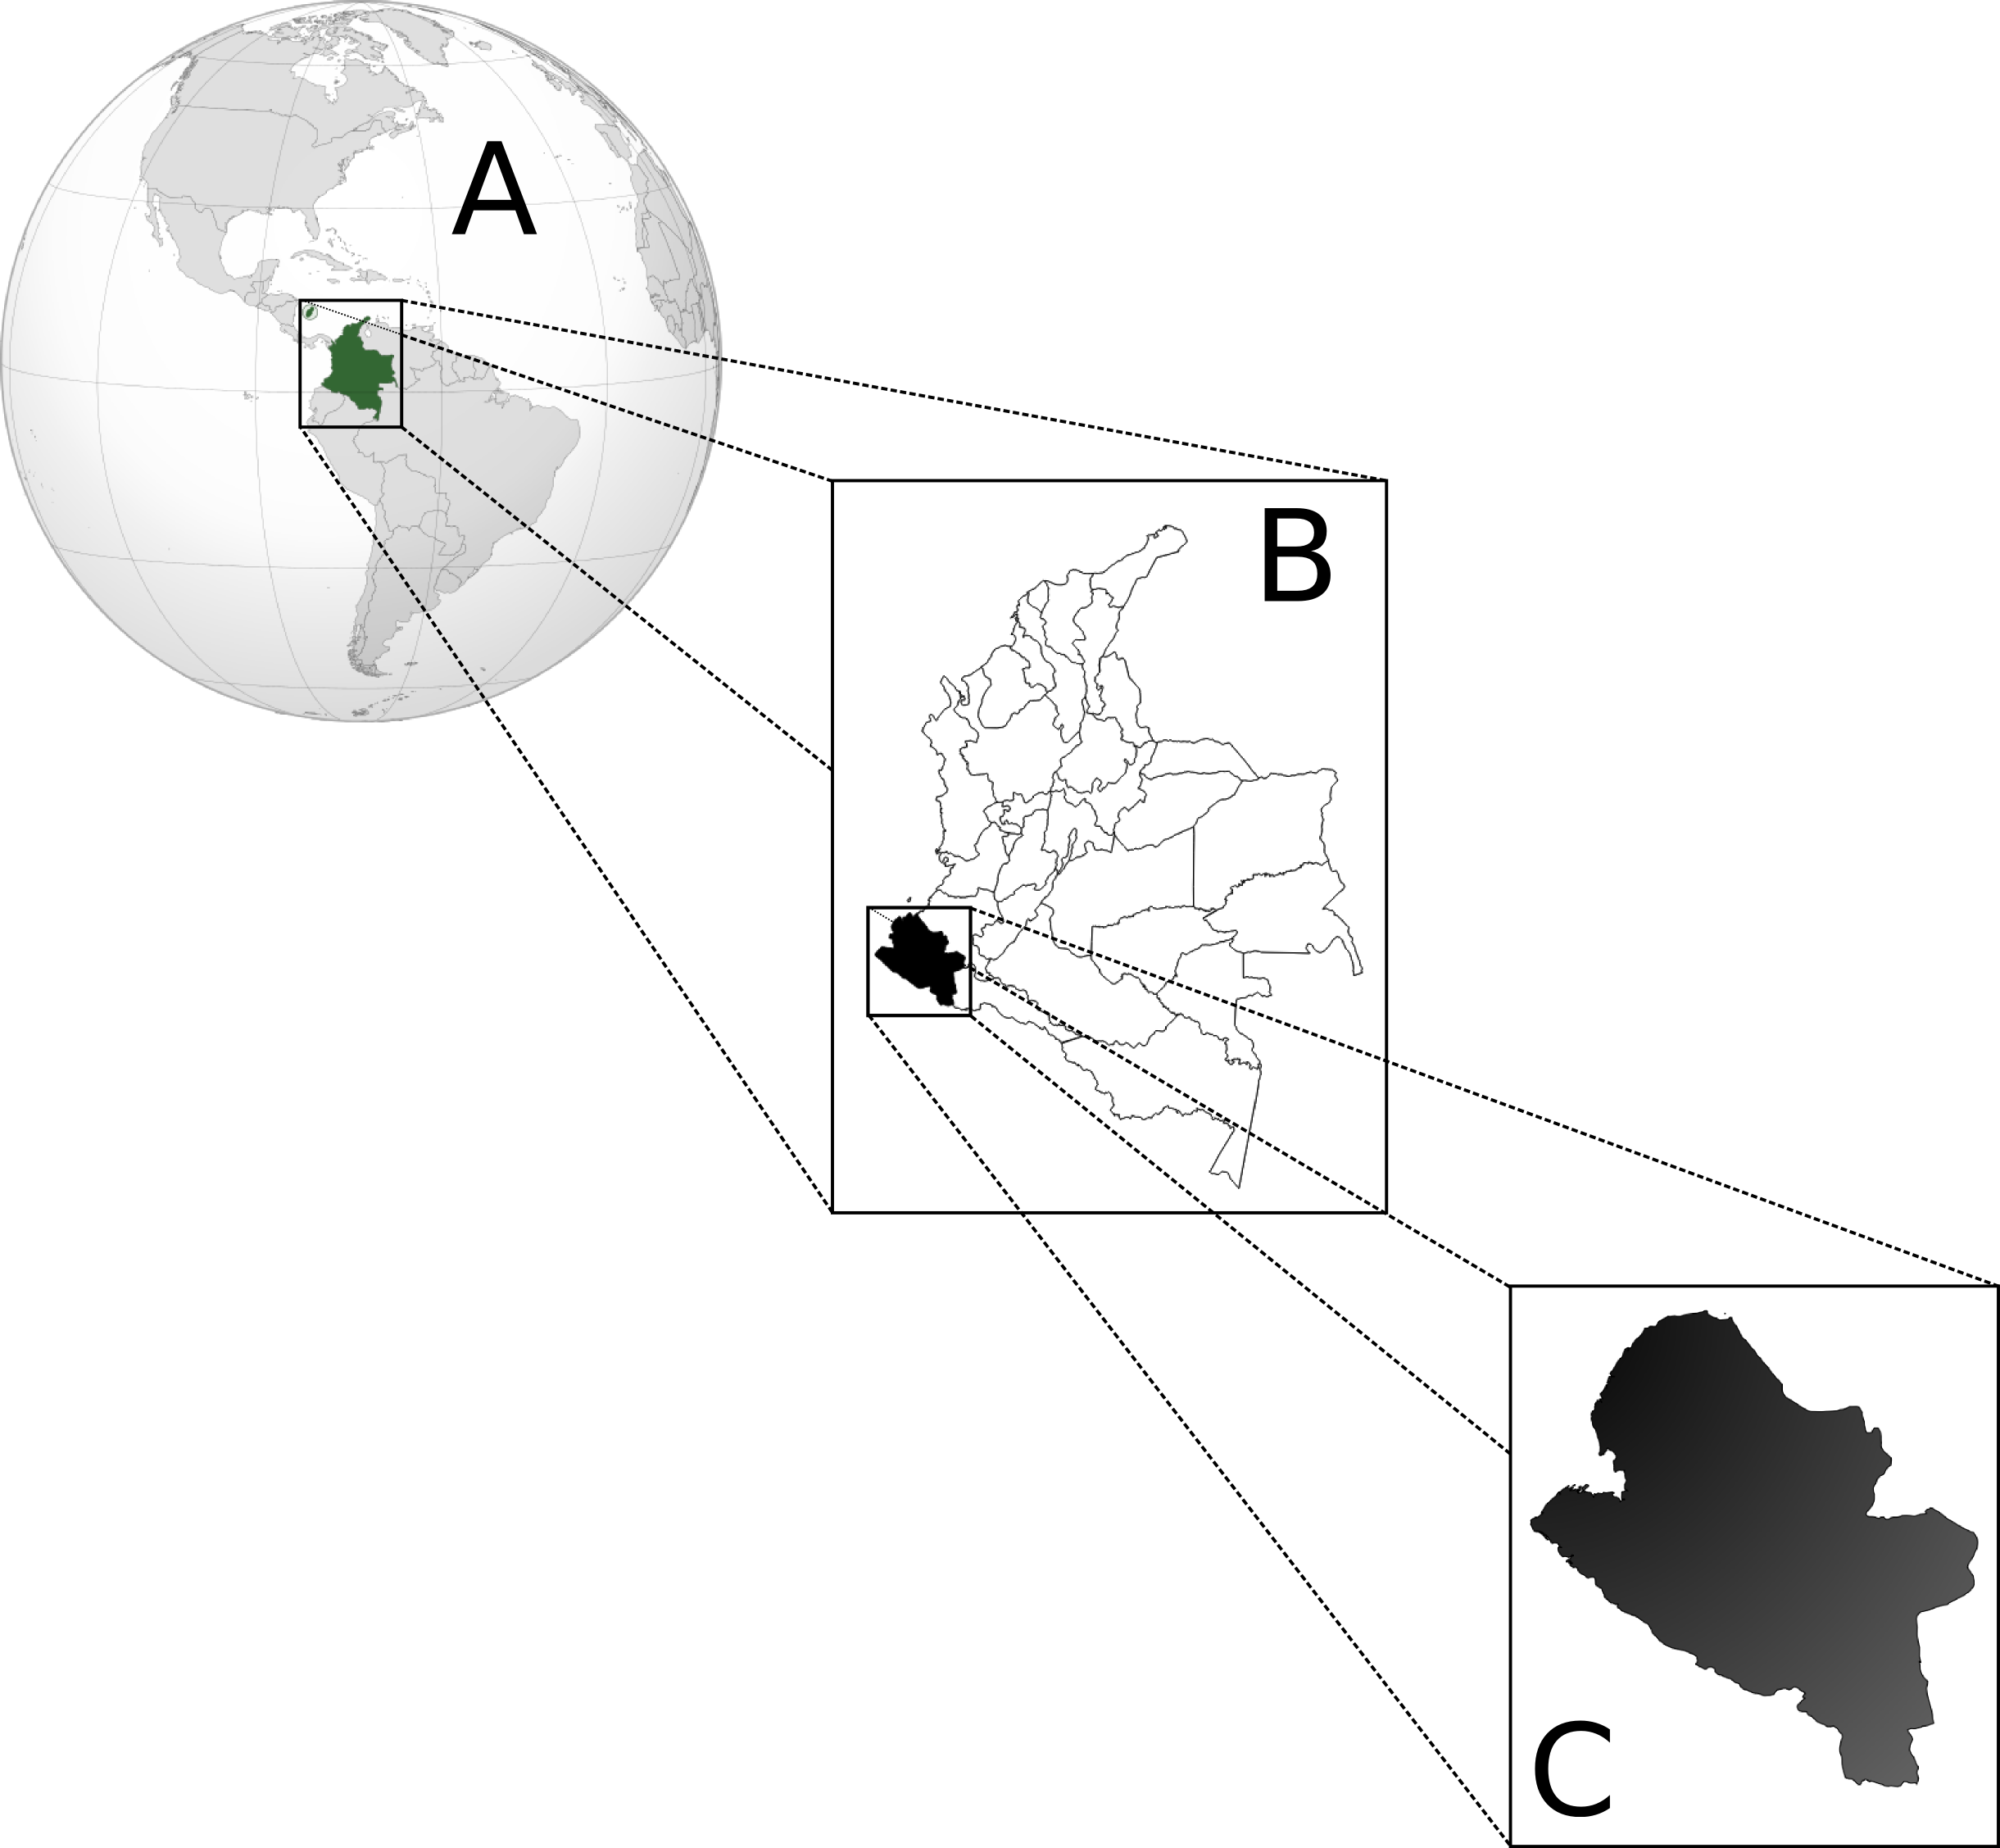
\includegraphics[width = 8cm]{locationNarino.png}
  \caption{Localización area de estudio}
  \label{fig:locationNarino}
\end{figure}
\section{Trabajos relacionados}

Diferentes estudios han explorado la construcción de mapas eólicos a partir
 de muestras tomadas en terreno.
 Por ejemplo, \cite{haslett1989spacetime} utilizan técnicas de auto-correlación espacio-temporal, para estimar la
 potencia generada por turbinas en Irlanda a partir de pocos datos de entrada.
 Adicionales técnicas de interpolación espacial fueron utilizadas por \cite{luo2008acomparison} 
 para generar mapas de viento de alta resolución en el Reino Unido.
 El objetivo perseguido por la investigación era comparar y evaluar diversos
 métodos de interpolación para seleccionar el más adecuado.
 En los Países Bajos, \cite{stepek2011interpolating}  utilizan un modelo llamado de bicapa para estimar la velocidad del viento
 a partir de 31 estaciones meteorológicas.

Sin embargo, es importante resaltar que las características de velocidad
 y dirección del viento no son lo únicos criterios a tener en cuenta a la
 hora de escoger las mejore ubicaciones.
 La evaluación multi-criterio (MCE) ha tenido una amplia acogida a la hora
 de evaluar características físicas junto con otros atributos como aspectos
 económicos y sociales.
 
\cite{rodman2006ageographic}  utilizan técnicas MCE para determinar posibles ubicaciones de turbinas
 en el norte de California evaluando componentes físicos,ambientales y humanos. \cite{janke2010multicriteria}
 categoriza diferentes aspectos de acuerdo al potencial eólico y solar e
 identifica áreas susceptibles a la instalación de turbinas y paneles solares
 en Colorado.
 
 Entre los aspectos evaluados se encuentran la distancia a carreteras y
 líneas de transmisión eléctrica, coberturas del terreno, densidad de población
 y áreas protegidas por la ley. \cite{petrov2014utilization} explora nuevos algoritmos de análisis de datos para modelar la ubicación
 de turbinas en Iowa apoyándose en un sistema espacial multi-criterio de
 soporte a la toma de decisiones.
 Nuevas técnicas de análisis de datos, comúnmente conocidas como minería
 de datos, han demostrado muy buenos resultados a la hora de modelar fenómenos
 atmosféricos.
 
 Por ejemplo, \cite{yusof2014miningfrequent} utiliza algoritmos para detectar patrones secuenciales en series de tiempo
 de viento desde estaciones en los Países Bajos para detectar anomalías
 en el flujo, velocidad y dirección del viento.



\section{Metodología}

La metodología usada para la construcción del mapa de irradiacin solar se la puede ver en la figura~\ref{fig:metodology}

\begin{figure}
  \centering
  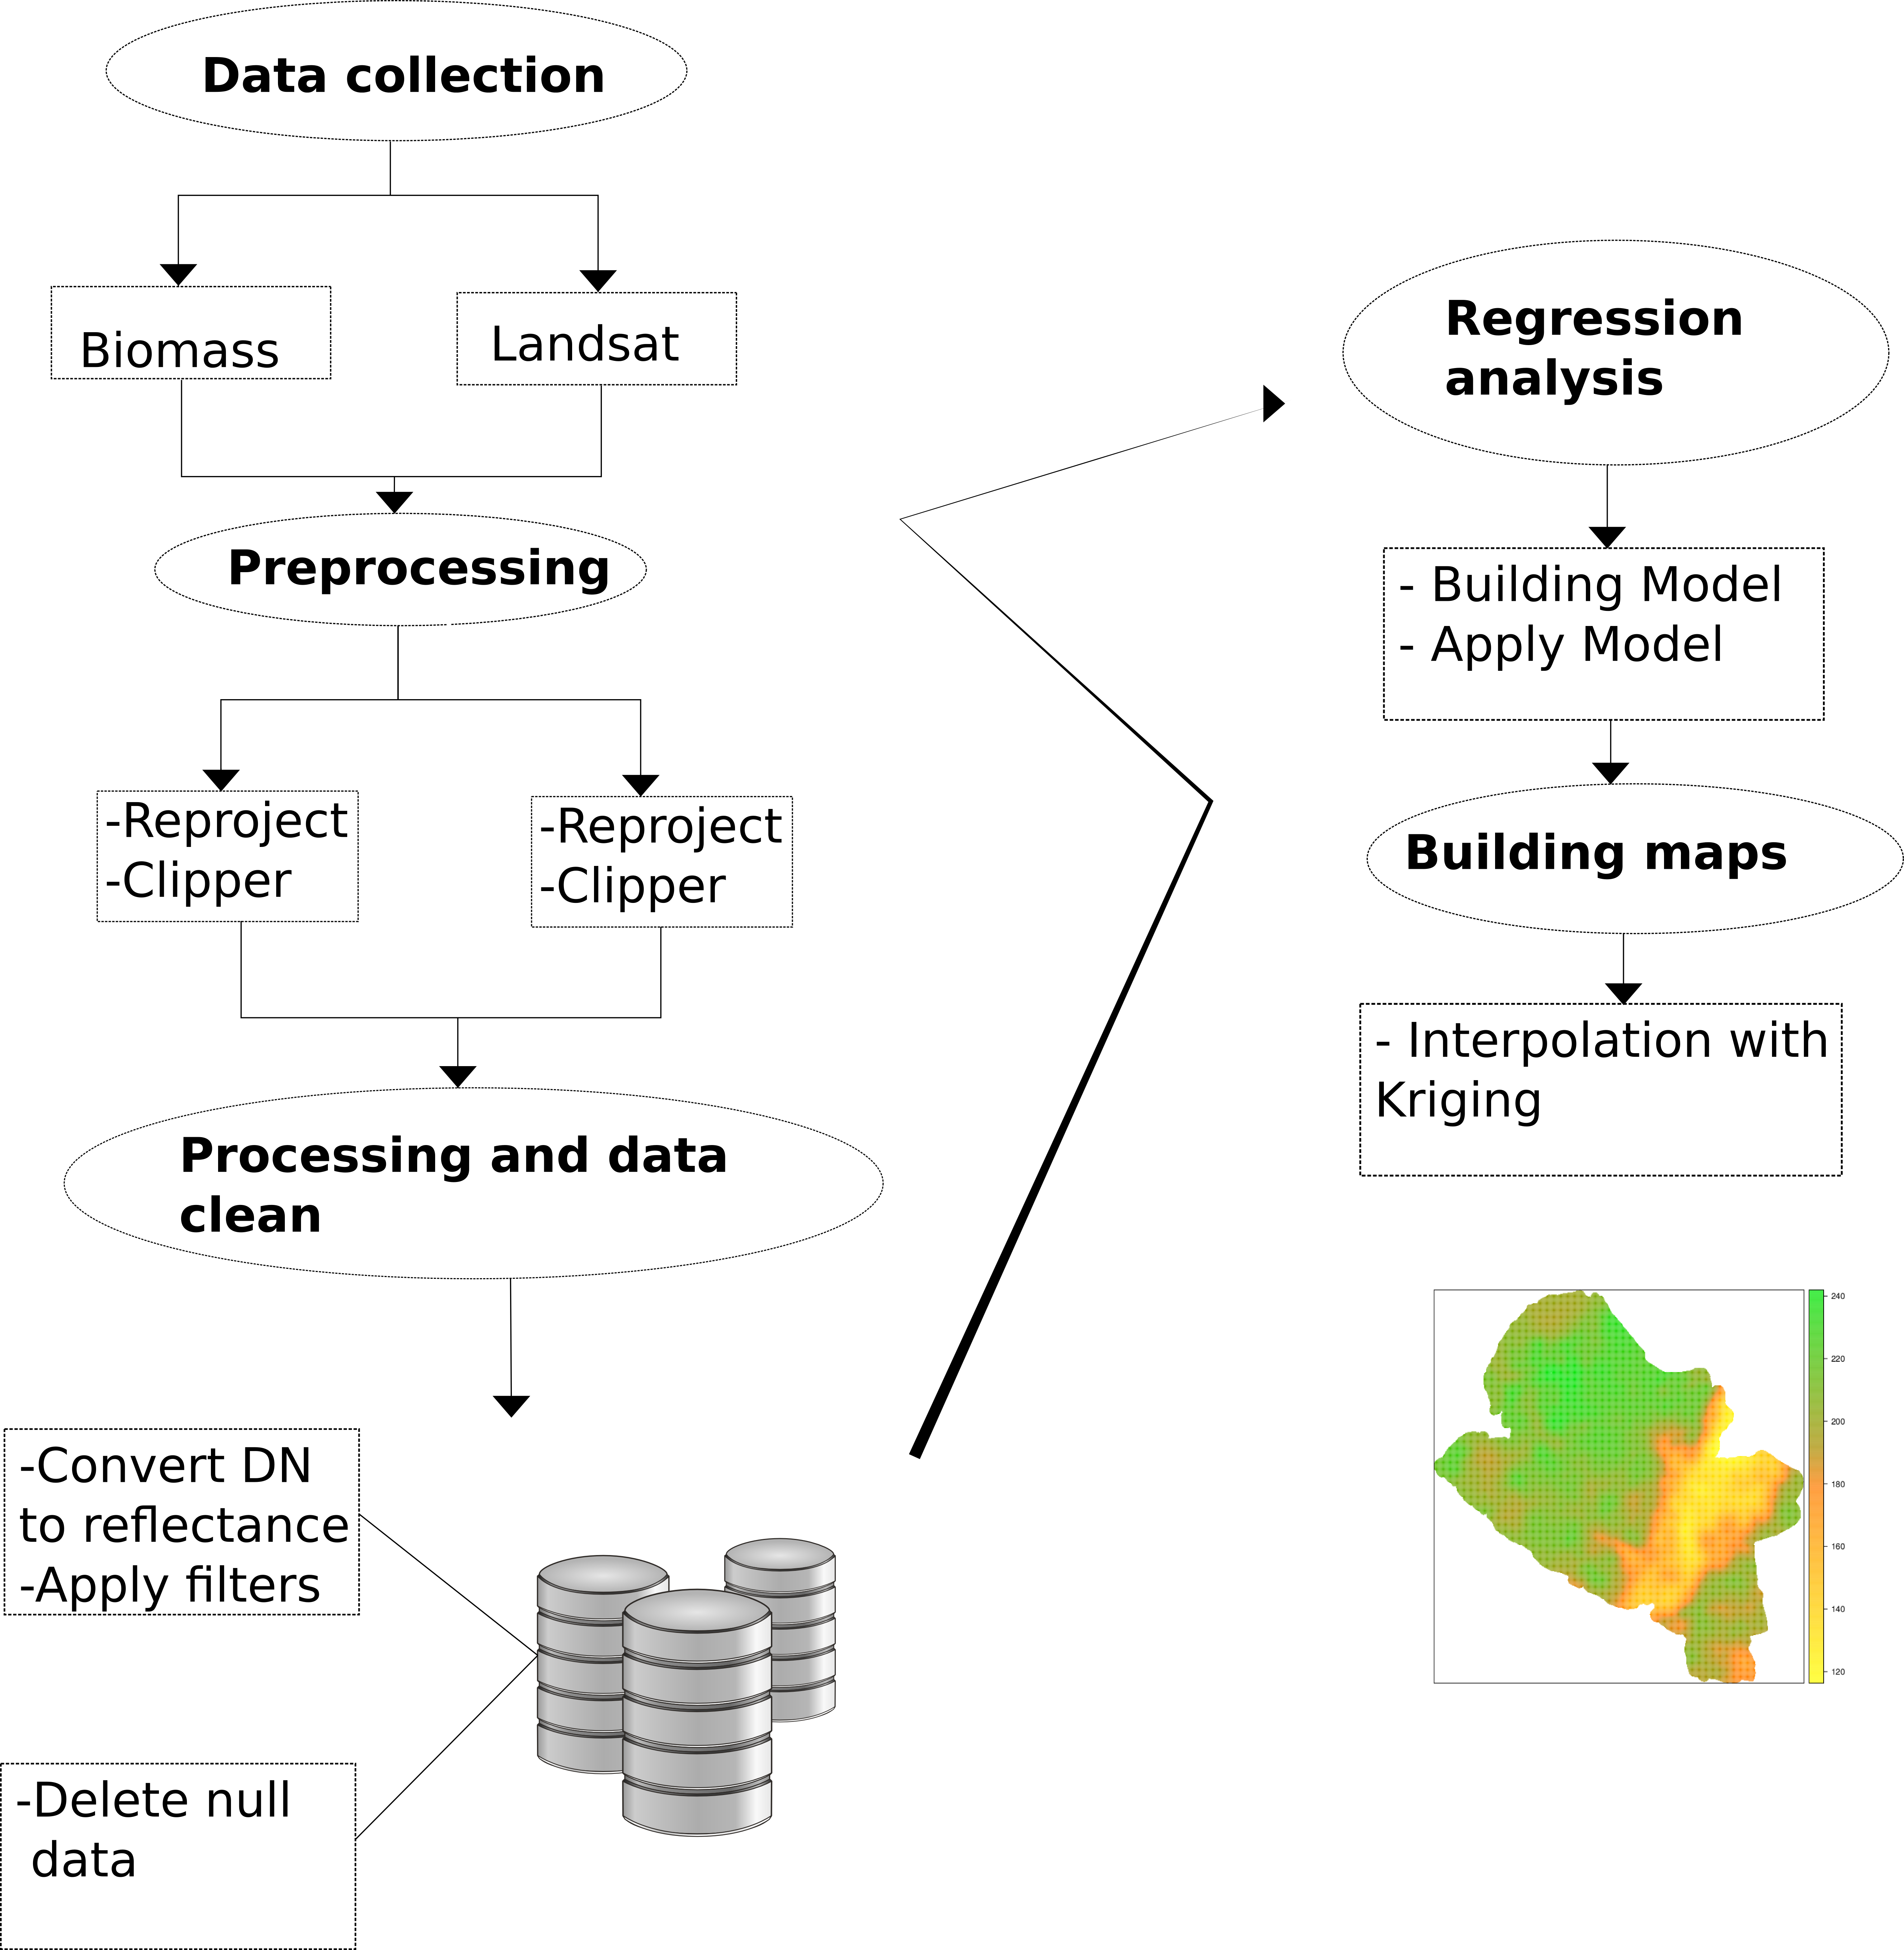
\includegraphics[width = 8cm]{metodology.png}
  \caption{Metodología}
  \label{fig:metodology}
\end{figure}

\subsection{Obtención de datos}

El proceso de obtención de datos se realizó tomando imágenes satelitales que provee el satélite
Landsat 7. En este proceso se descargaron 1362 imágenes satelitales desde el año 1999 hasta el año 2015, que cubren el 
departamento de Nariño. Para cubrir todo el departamento fue necesario descargar las imagenes satelitales con 
los siguientes paths y rows: (009,059), (009,060), (010,058), (010,059), (011,059) 

En la obtención de datos también se utilizó el mapa de irradiancia solar proporcionado por VAISALA INC (3TIER).

\subsection{Preprocesamiento}

En esta etapa de preprocesamiento se reproyecto las imágenes obtenidas, debido a que las cinco imágenes
que cubren el departamento de Nariño, estan en distintos sistemas de coordenadas (EPSG:32618 y EPSG:32617) y se 
lo reproyecto al sitema EPSG:3857. Así como también se recorto las imágenes con el fin de unicamente tener 
el área que cubre el departamento de Nariño, como lo muestra la figura~\ref{fig:Recortar imágenes}

\begin{figure}
  \centering
  \subfigure[Imágenes Satélitales de Nariño]{\label{Imágenes Satélitales Nariño} 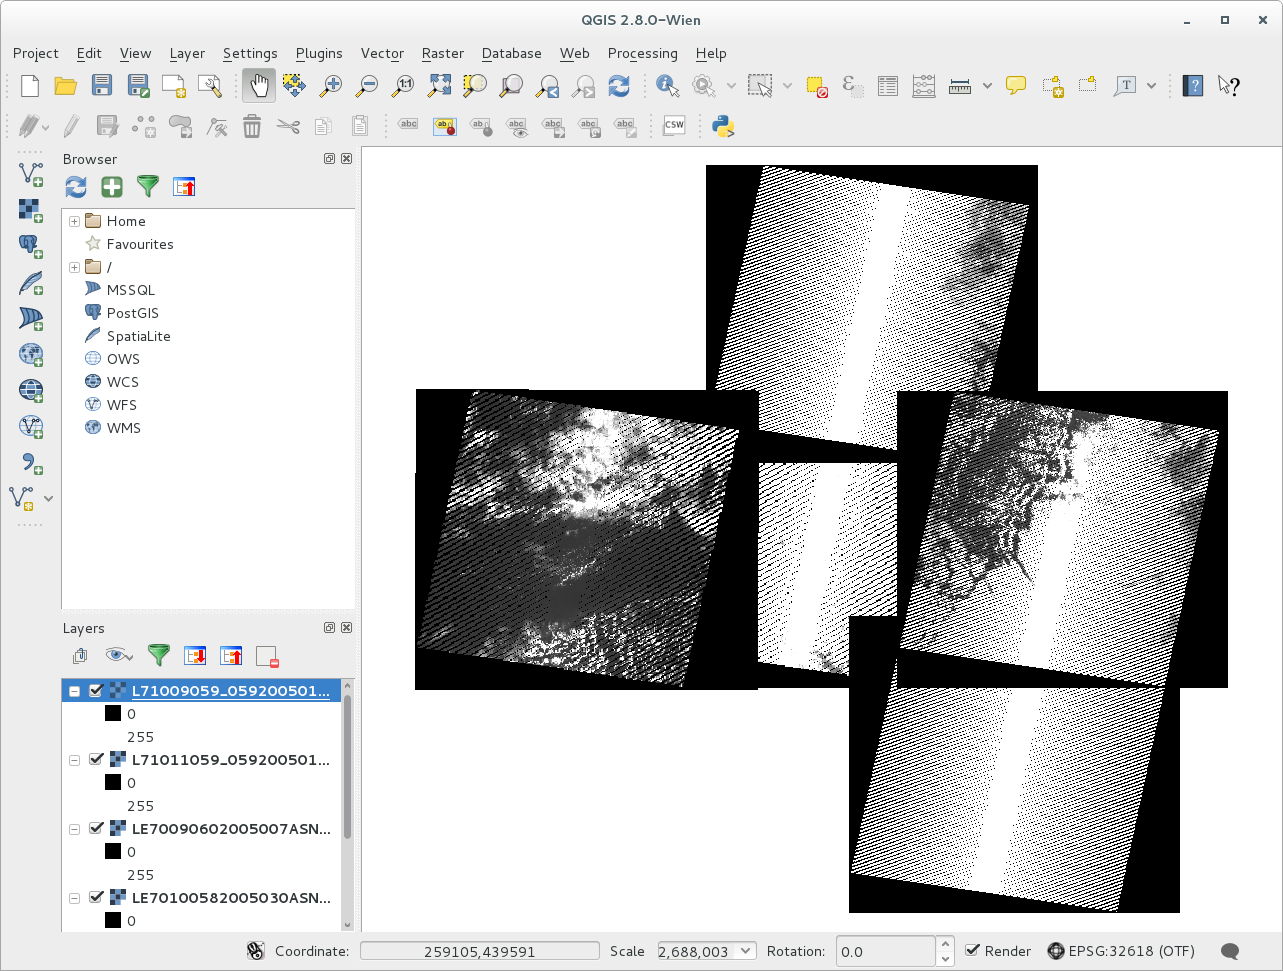
\includegraphics[width= 7cm]{cut1.png}}
  \vfill
  \subfigure[Imágenes recortadas de Nariño]{\label{Imágenes recortadas de Nariño}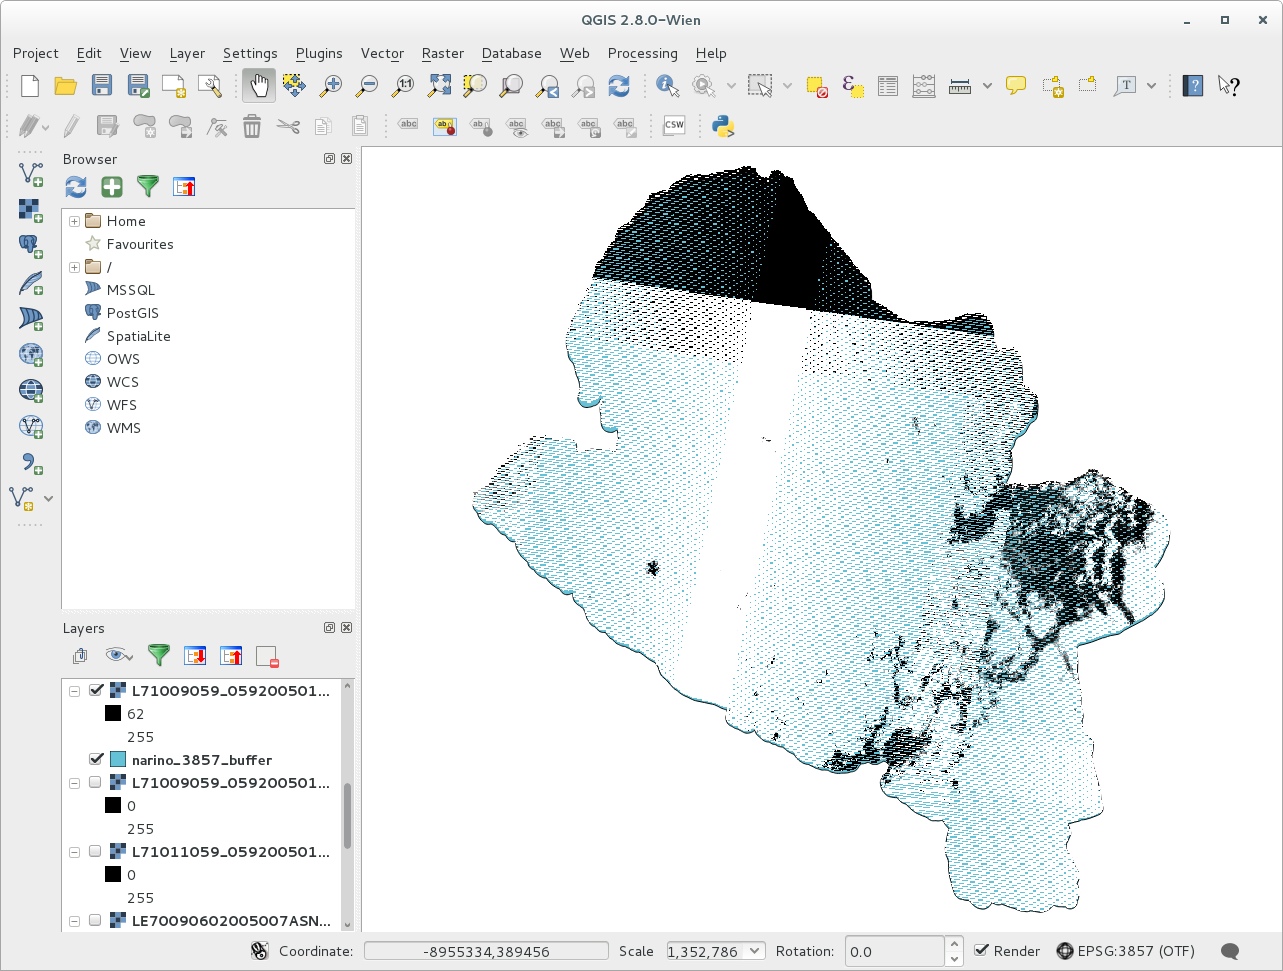
\includegraphics[width= 7cm]{cut2.png}}
  \caption{Prepocesamiento}
  \label{fig:Recortar imágenes}
\end{figure}

De igual manera este proceso se lo realizó para el mapa de biomasa, como se muestra en la figura~\ref{fig:mapaNarino}


\subsection{Procesamiento y limpieza de datos}

Se diseñó una base de datos para capturar los datos,
como lo muestra la figura~\ref{fig:landsatET}, la cual tiene 4 tablas. 

\begin{figure}
  \centering
  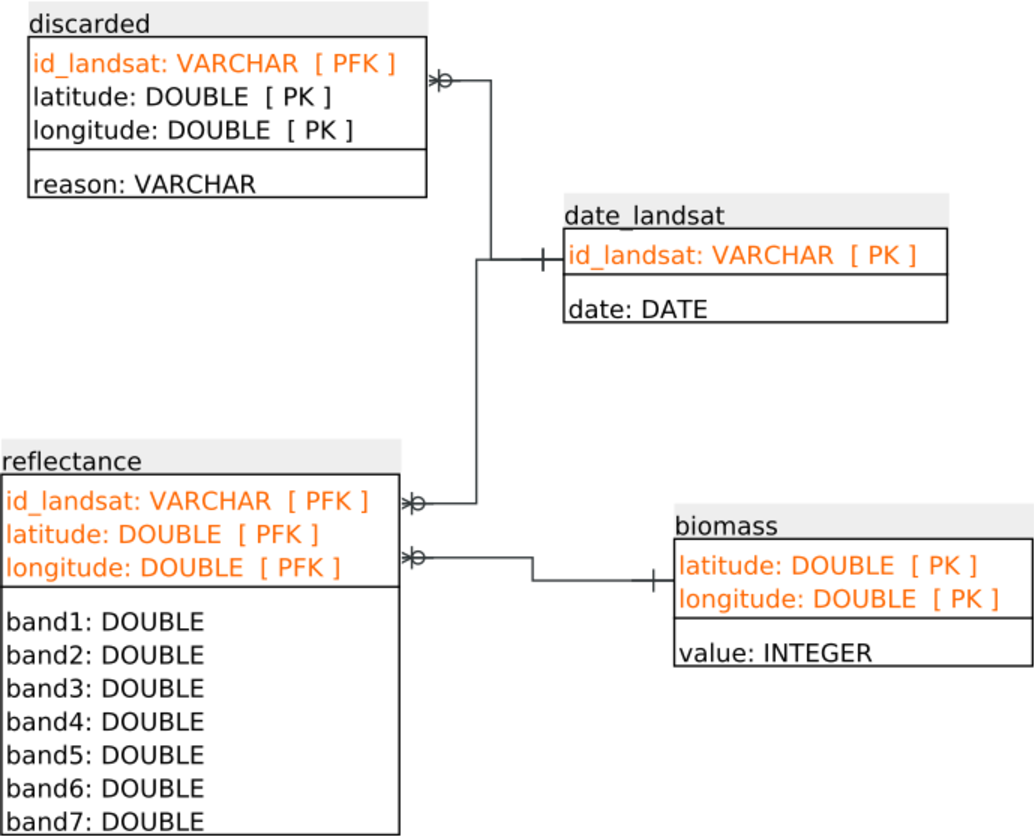
\includegraphics[width = 8cm]{landsatET.pdf}
  \caption{Modelo entidad-relacion Landsat}
  \label{fig:landsatET}
\end{figure}

Tabla date\_landsat: en la cual se almacenan las fechas de las imágenes satelitales.

Tabla reflectance: en la cual se almacenan los datos capturados y convertidos en reflentance,
de las bandas landsat (1 - 5,7) y la temperatura en grados kelvin de la banda 6.

Tabla discarded: en la cual se almacenan datos que fueron descartados, por varias razones,
son nubes calientes, nubes frias, datos ambiguos o no son vegetación.

Tabla biomass: en la cual se almacenan los datos de biomassa del mapa de \cite{baccini2008afirst}.

Para procesar las imágenes y llenar la base de datos se realizó un Script, el cual captura el Digital Number
de las imágenes satélitales y lo transforma en valor en reflectance. En este procesamiento de imagenes, se adiciono al Script unos filtros para para detección de nubes calientes,
nubes, frias, datos ambiguos como lo muestra el algoritmo propuesto por \cite{irish2000landsat}, además se aplico 
un filtro adicional, el NVDI(normalized difference vegetation index) para trabajar unicamente con datos de vegetación.

La tabla~\ref{tab:datos} muestra la relación de los datos obtenidos en este proceso.

\begin{table}
\caption{Datos obtenidos en en el proceso de procesamiento y limpieza  de datos}
\label{tab:datos}
\centering
\scalebox{0.7}{
\begin{tabular}{c c c}
\toprule
 Nombre & Valor& Detalle  \\
\midrule
Imágenes landsat procesadas & 1321 & Imágenes de Nariño de 2000 a 2014 \\
Datos Totales & 51.076.512 & Registros Totales desde año 2000 a 2014 \\
Datos biomasa & 81.993 & Registros de biomasa para año 2000 a 2003 de  \cite{baccini2008afirst}\\
Nube caliente & 3.731.768 & Registros de 2000 a 2014 \\
Nube Fria & 27.827.009 & Registros de 2000 a 2014 \\
No vegetacion & 3.459.210 & Registros de 2000 a 2014 \\
Ambiguo & 11.987.340 & Registros de 2000 a 2014 \\
Datos Validos Reflectance & 4.071.185 & Registros de 2000 a 2014 \\
\bottomrule
\end{tabular}}
\end{table}

\subsection{Análisis de regresión}

El análisis de regresión se realizó tomando los valores de las bandas landsat obtenidas año 2000 y 2003 y el valor de biomasa obtenido en \cite{baccini2008afirst},
para poder obtener un mejor modelo se agrupó y se saco un promedio con valores de las bandas landsat en cada punto, se fue iterando con  valores que superaban al menos N número de
muestras, siendo N desde 1 hasta 45 muestras, el mejor modelo obtenido fué cuando el número de muestas en cada punto superaba al menos las 35 muestras, este conjunto
de datos obtenido tenía 1009 registros. El comportamiento en las demás iteraciones muestra que con menos muestras hay más registros y eso hace que no se encuentre un buen modelo,
pero cuando hay mas muestras los registros son menores y esto también hace que el resultado del modelo tampoco sea bueno.

En la tabla~\ref{tab:metricas} se muestra las métricas de los modelos analizadas con 35 muestras y 1009 datos, el cual es el mejor modelo, esta tabla 
se la realizó usando la biblioteca de código abierto rminer presentada por \cite{cortez2010data} para la herramienta R.

\begin{table}
\caption{Métricas de modelos analizados con datos de Landsat}
\label{tab:metricas}
\centering
\scalebox{0.7}{
\begin{tabular}{c c c c c c c}
\toprule
 & SAE& MAE & RAE & RMSE & COR & R2 \\
\midrule
ctree & 771.66185 & 5.32181 & 33.37397 & 8.89544 & 0.85991 & 0.73945 \\
rpart & 819.97501 & 5.65500 & 35.4634 & 9.23174 & 0.84774 & 0.71865 \\
kknn & 583.3615 & 4.02318 & 25.23008 & 6.19161 & 0.93584 & 0.87580 \\
mlp & 558.43603 & 3.85128 & 24.15206 & 5.49114 & 0.94968 & 0.90189 \\
mlpe & \textbf{461.93253} & \textbf{3.18574} & \textbf{19.97834} & \textbf{4.73616} & \textbf{0.96292} & \textbf{0.92721} \\
ksvm & 574.76656 & 3.96391 & 24.85835 & 5.71528 & 0.94664 & 0.89613 \\
randomForest & 663.70528 & 4.57728 & 28.70490 & 6.89480 & 0.92117 & 0.84856 \\
mr & 752.19550 & 5.18756 & 32.53206 & 6.75745 & 0.92222 & 0.85049 \\
mars & 680.67053 & 4.69428 & 29.43864 & 6.34212 & 0.93186 & 0.86837 \\
cubist & 538.20590 & 3.71176 & 23.27712 & 6.34056 & 0.93141 & 0.86752 \\
plsr & 748.89239 & 5.16478 & 32.38920 & 6.76538 & 0.92208 & 0.85023 \\
cppls & 748.89239 & 5.16478 & 32.38920 & 6.76538 & 0.92208 & 0.85023 \\
\bottomrule
\end{tabular}}
\end{table}

\begin{table}
\caption{Métricas de modelos analizados con datos de MODIS}
\label{tab:metricas}
\centering
\scalebox{0.7}{
\begin{tabular}{c c c c c c c}
\toprule
 & SAE& MAE & RAE & RMSE & COR & R2 \\
\midrule
ctree & 1360.88975 & 9.13349 & 60.07076 & 13.06545 & 0.64264 & 0.41299 \\
rpart & 1373.21922 & 9.21624 & 60.61499 & 14.14182 & 0.60074 & 0.36089 \\
kknn & 920.48535 & 6.17775 & 40.63096 & 10.31934 & 0.79280 & 0.62854 \\
mlp & 485.60361 & 3.25908 & 21.43493 & 4.51435 & 0.96284 & 0.92705 \\
mlpe & 443.11836 & 2.97395 & 19.55960 & 3.97730 & 0.97157 & 0.94394 \\
ksvm & 823.63424 & 5.52775 & 36.35587 & 8.12712 & 0.87861 & 0.77195 \\
randomForest & 1159.07988 & 7.77906 & 51.16271 & 11.04659 & 0.75129 & 0.56444 \\
mr & 597.58282 & 4.01062 & 26.37778 & 5.36391 & 0.94694 & 0.89670 \\
mars & 618.82261 & 4.15317 & 27.31532 & 5.47634 & 0.94475 & 0.89255 \\
cubist & 597.29188 & 4.00867 & 26.36494 & 5.36508 & 0.94688 & 0.89658 \\
plsr & 597.29188 & 4.00867 & 26.36494 & 5.36508 & 0.94688 & 0.89658 \\
cppls & 597.29188 & 4.00867 & 26.36494 & 5.36508 & 0.94688 & 0.89658 \\
\bottomrule
\end{tabular}}
\end{table}

En este proceso tambien se usó el paquete R Boruta \cite{kursa2010feature}, el cual es un nuevo algoritmo de selección de características 
para encontrar todas las variables relevantes. El algoritmo está diseñado como un recubrimiento alrededor 
del algoritmo de clasificación random forest. Esto para saber si todas las bandas de landsat utilizadas eran relevantes para encontrar biomasa, 
en la figura~\ref{fig:boruta} se puede observar la relevancia de las bandas landsat para encontrar biomasa en el mejor modelo.

\begin{figure}
  \centering
  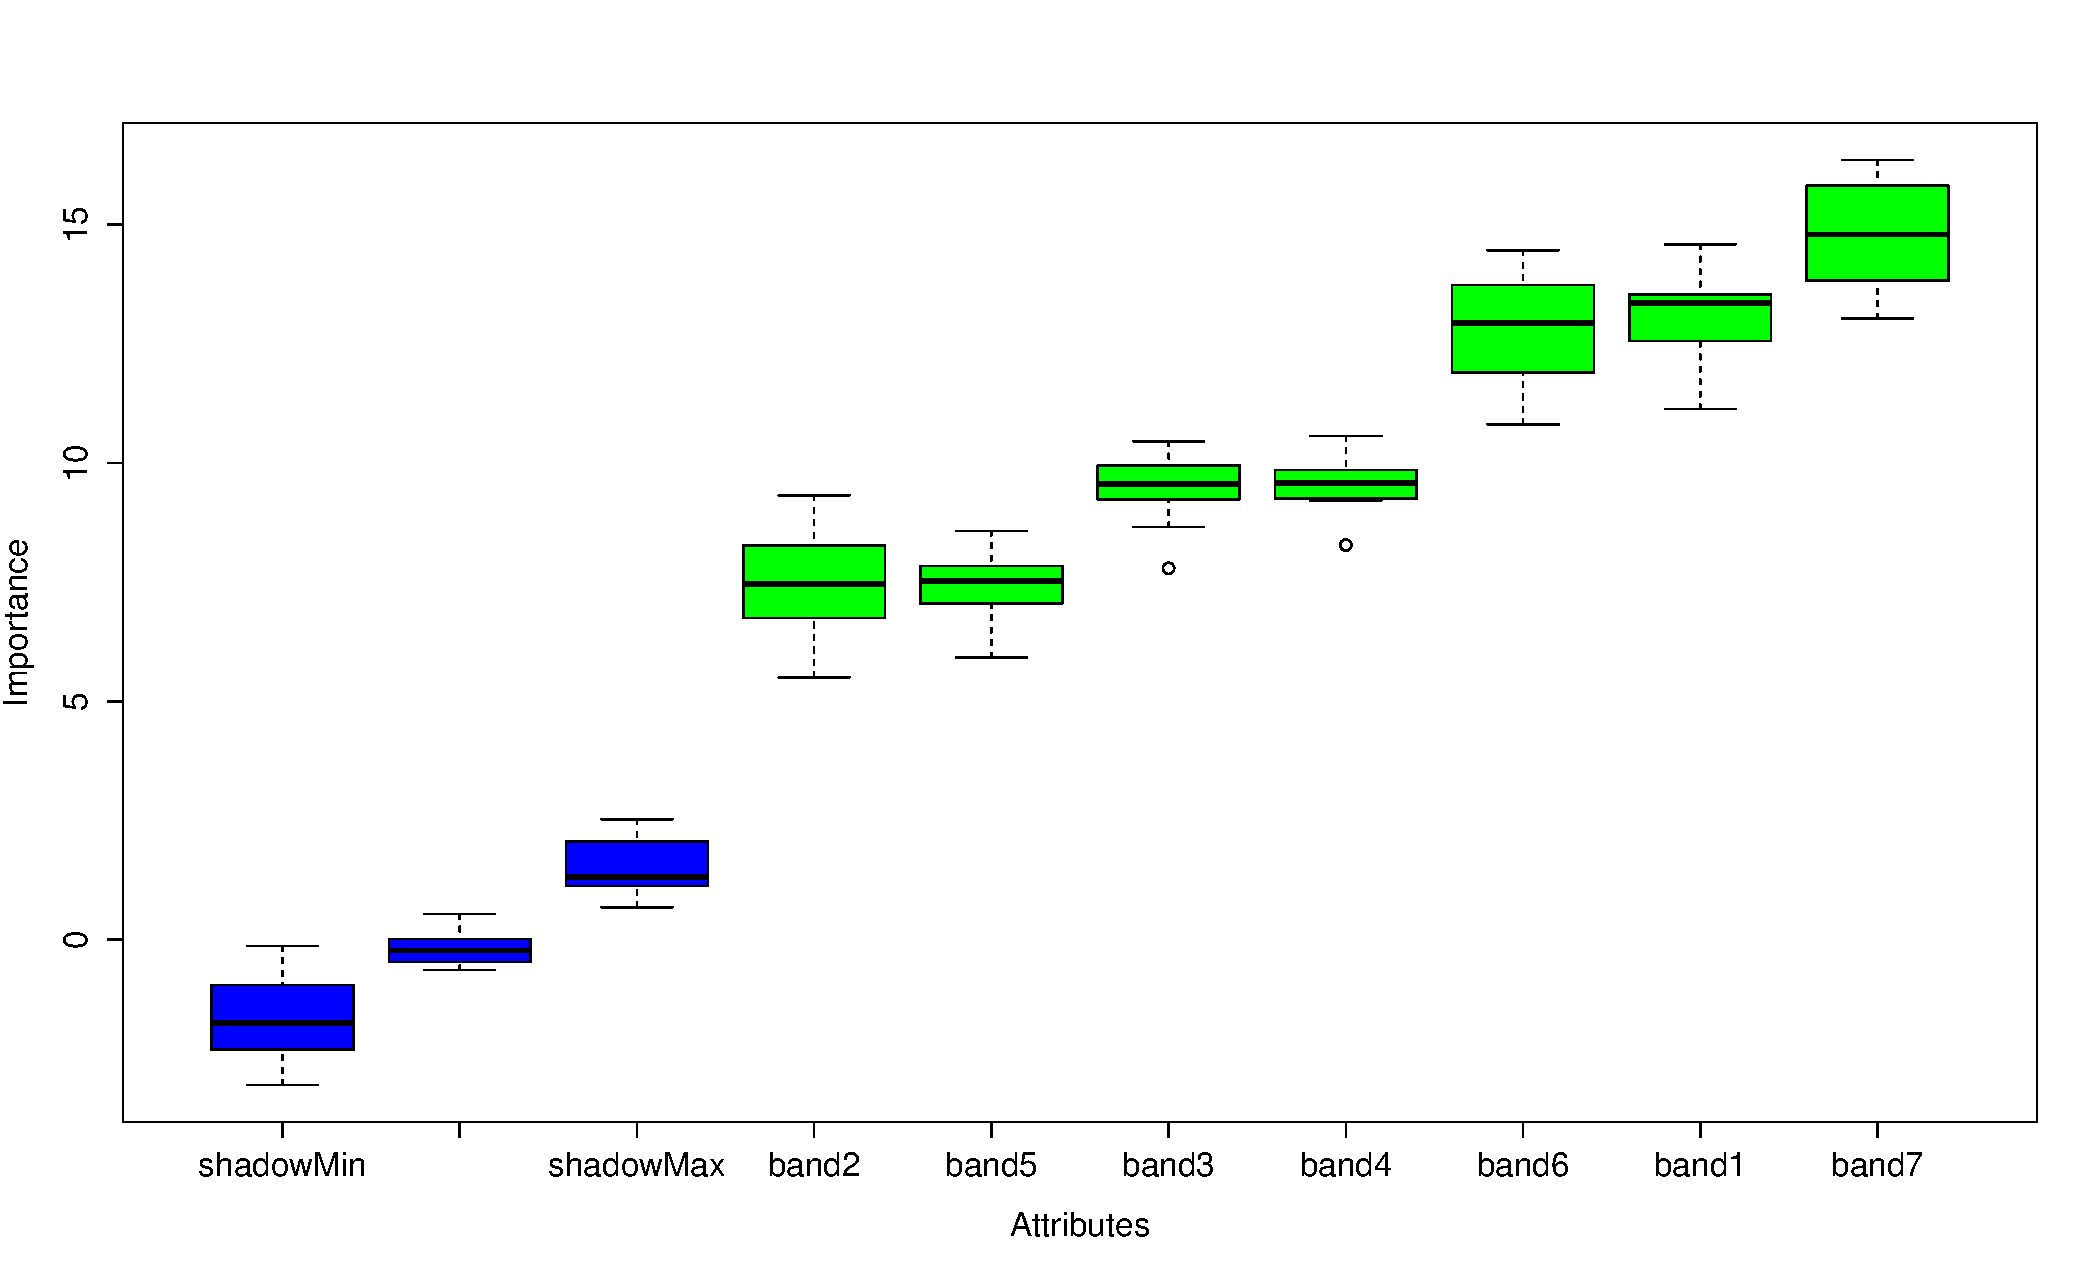
\includegraphics[width = 8cm]{boruta.pdf}
  \caption{Relevancia de bandas landsat en el análisis de regresión}
  \label{fig:boruta}
\end{figure}

\subsection{Construcción de mapas}

Para la construcción de mapas de biomasa se utilizó el método Kriging que provee una solución al problema 
de la estimación basada en un modelo continuo de variación espacial estocástica, el objetivo de Kriging es el de estimar el valor de una 
variable aleatoria, Z, en uno o más puntos no muestreados o sobre grandes bloques. 

El método Kriging recibe como entrada datos de la muestra, y una malla dependiendo de la resolución que se quiera obtener, por ello los datos de muestra se
obtuvieron aplicando el modelo obtenido en el análisis de regresión a datos agrupados en cada punto por mes, año y uno general entre el año 2000 a 2014; y la 
 malla se construyó con puntos regulares espaciados cada 450 metros. 
 
 En la figura~\ref{fig:biomasaMes}, figura~\ref{fig:biomasaAnio}, figura~\ref{fig:biomasaTotal}  se muestra los mapas obtenidos por meses, años y general entre el año 2000 a 2014 respectivamente. 
 
\begin{figure}
  \centering
  \includegraphics[width = 8cm]{monthsLandsat.pdf}
  \caption{Mapas biomasa por meses}
  \label{fig:biomasaMes}
\end{figure}

\begin{figure}
  \centering
  \includegraphics[width = 8cm]{yearsLandsat.pdf}
  \caption{Mapas biomasa por años}
  \label{fig:biomasaAnio}
\end{figure}

\begin{figure}
  \centering
  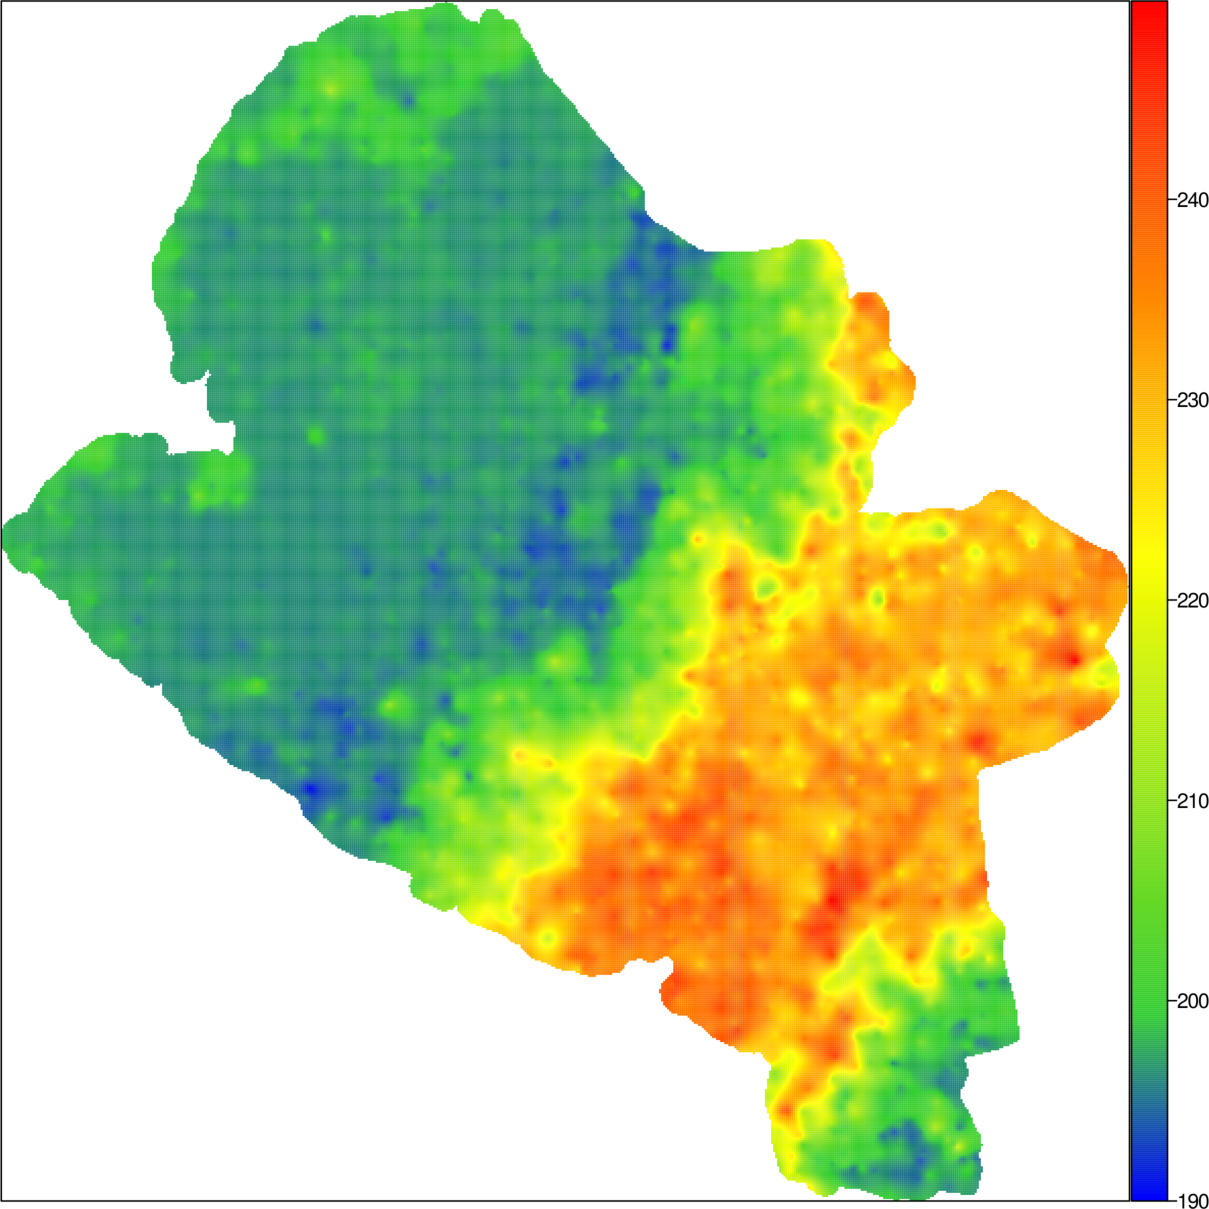
\includegraphics[width = 8cm]{generalLandsat.pdf}
  \caption{Mapas biomasa general años 2000-2014}
  \label{fig:biomasaTotal}
\end{figure}

\section{Conclusiones}

Se construyeron mapas energéticos con el componente solar en el departamento de Nariño,
usando los sensores Landsat 7 y MODIS.

Las imágenes sateliatles son una gran fuente de información debido a la capacidad de almacenar gran cantidad de registros históricos para diferentes tipos de datos, estos datos
poco a poco estan siendo utilizados por organizaciones para determinar características terrestres, fenómenos naturales, condiciones de los mares,
características de la vegetación, etc. Por esta razón el uso de imágenes satelitales
en la investigación da resultados aproximados y a bajo costo, teniendo en cuenta el costo
que puede implicar hacer muestreo en campo.

Se construyo una metodología para la construcción de mapas energéticos con el potencial
de radiación solar, el cual se lo puede aplicar en zonas donde no tengan estaciones climáticas con los sensores Landsat o MODIS.

En la construcción del mejor modelo, con ambos sensores Landsat 7 y MODIS se tubo un $R^2$ por encima del 90\%,
teniendo en cuenta que las imágenes landsat 7 se obtienen cada 16 dias y las de MODIS son diarias, sería
de mayor provecho usar el sensor MODIS para hacer estudios posteriores con series de tiempo.

Tanto la correlación como el $R^2$ entre los mapas construidos a partir del sensonr Landsat 7 y MODIS
es buena, teniendo en cuenta que en el mapa general se tiene una correlación del 94\% y un $R^2$ del
88\%.



%\appendices
%\section{Repositorio}
%El código fuente y conjunto de datos se encuentran en el repositorio de github.


\ifCLASSOPTIONcompsoc
  % The Computer Society usually uses the plural form
  \section*{Agradecimientos}
\else
  % regular IEEE prefers the singular form
  \section*{Agradecimientos}
\fi

Universidad de Nariño, Universidad de los Andes y Sistema de Regalias.

% Can use something like this to put references on a page
% by themselves when using endfloat and the captionsoff option.
\ifCLASSOPTIONcaptionsoff
  \newpage
\fi


\bibliographystyle{IEEEtran}

\bibliography{IEEEabrv,bibliography}



\end{document}
